% Partie en ligne (Younes Bensallah) : recherches, classement, recommandations,
% API, client et mesures en ligne.
\section{Partie en ligne : recherche, classement et recommandations}
\label{sec:enligne}

Les trois recherches suivent le même schéma : chacune calcule un nombre
d'occurrences par livre, sous la forme d'une table $\mathit{occ} : \text{livre}
\to \mathbb{N}$, puis un module commun trie, découpe en pages et ajoute les
suggestions (section~\ref{sec:classement}). Changer de tri ou ajouter une
recherche ne touche donc qu'une pièce.

\subsection{Recherche par mot-clé dans l'index inversé}
\label{sec:motcle}

\paragraph{Problème et structure de données.} Étant donnée une requête
$q = w_1 \dots w_k$, renvoyer, comme le demande le sujet, les livres dont la
table d'index contient chaque $w_i$ \emph{tel quel} : \motif{prin} ne trouve
ni \motif{prince} ni \motif{princess} ; pour les variantes d'un mot, on passe à
la RegEx \motif{prin.*} sur l'index (section~\ref{sec:regexindex}). La requête
passe par le même découpage que les livres, et l'index inversé est la table
\texttt{occurrence} de la section~\ref{sec:index} : sa clé primaire
$(\mathit{term\_id}, \mathit{book\_id})$ est un arbre B, donc la liste de
\emph{postings} d'un terme se lit par un seul parcours d'intervalle, et un
second arbre B sur \texttt{term.word} donne le numéro d'un mot.

\paragraph{Algorithme.} La sémantique est un ET : un livre est retenu s'il
contient les $k$ mots, et son score est la somme de leurs fréquences. En SQL,
on lit les $k$ listes de postings (\texttt{t.word = ANY(?)}), on groupe par
livre et on garde les groupes de taille $k$ (\texttt{HAVING count(*) = k}). Le
coût est $O(\sum_i |P(w_i)|)$, où $|P(w)|$ est la longueur de la liste
de $w$ (au plus 2000), plus $k$ descentes dans l'arbre B des termes : il ne
dépend pas de la taille des textes.

\paragraph{État de l'art et choix.} L'index inversé est la structure de
référence de la recherche textuelle~\cite{zobel,iir}. Les moteurs spécialisés
(Lucene, Elasticsearch) compressent les listes de postings (codage delta,
\emph{variable byte}) et les intersectent par fusion, en commençant par la plus
courte et en sautant des blocs (\emph{skip lists}, recherche galopante). Avec
au plus 2000 entrées par liste, PostgreSQL suffit, et garder l'index dans une
table SQL permet de le lire aussi bien par terme (recherche) que par livre
(calcul de Jaccard). Le score par nombre d'occurrences est celui du sujet ; il
favorise les livres longs, ce que corrigerait tf-idf ou BM25~\cite{bm25}
(section~\ref{sec:conclusion}).

\subsection{Recherche par RegEx sur l'index}
\label{sec:regexindex}

\paragraph{Problème.} Étant donnée une RegEx $R$ (syntaxe d'\texttt{egrep} :
lettres, \motif{.}, \motif{|}, \motif{*}, \motif{+}, parenthèses), renvoyer les
livres dont la table d'index contient un terme $t \in L(R)$. Le score d'un livre
est la somme des fréquences des termes reconnus.

\paragraph{Algorithme.} $R$ est passée en minuscules puis compilée en automate
déterministe minimal (DFA) par la méthode développée au projet~1~\cite{projet1}.
Ce DFA teste ensuite chaque terme du
vocabulaire \emph{en entier} (\texttt{Dfa.accepte}) : \motif{sarg(o|a)n} reconnaît
\motif{sargon}, mais \motif{sarg} ne reconnaît rien, car ce n'est qu'un préfixe.
Le vocabulaire (517\,845 termes) est chargé une fois en mémoire, dans deux
tableaux rangés par nombre de livres décroissant ; le parcours est parallèle.
Les identifiants des termes reconnus sont envoyés à PostgreSQL en une seule
requête (\texttt{term\_id = ANY(?)}, puis \texttt{GROUP BY book\_id}). Le coût
est $O(|R|)$ à $O(2^{|R|})$ pour la compilation (le DFA minimal des RegEx
usuelles a moins de 20 états), plus $O(\sum_t |t|)$ pour le parcours du
vocabulaire, plus la lecture des postings des termes reconnus.

\paragraph{Limite de 2000 termes.} Une RegEx large (\motif{.*}, \motif{a.*})
reconnaît des centaines de milliers de termes : la requête SQL lirait alors
presque tout l'index. Nous gardons au plus 2000 termes, les plus répandus
d'abord (ceux qui changent le plus le résultat), et l'interface signale la
troncature (\texttt{termsTruncated}).

\paragraph{État de l'art et choix.} Lucene fait la même chose plus
efficacement~\cite{lucene} : son dictionnaire de termes est un automate
(FST) et il calcule l'\emph{intersection} des deux automates, ce qui élague
d'un coup tous les termes qui partagent un préfixe rejeté. Notre parcours
linéaire du vocabulaire est plus simple et reste de l'ordre de la dizaine de
millisecondes (figure~\ref{fig:vocabulaire}) : un arbre radix ou un FST ne
serait rentable que pour un vocabulaire bien plus grand.

\subsection{Recherche par RegEx sur le texte intégral}
\label{sec:regextexte}

\paragraph{Problème.} Renvoyer les livres qui contiennent une \emph{occurrence}
de $R$ dans leur texte, c'est-à-dire un facteur d'une ligne qui appartient à
$L(R)$. Contrairement à la recherche sur l'index, une occurrence peut couvrir
plusieurs mots (\motif{of.the.k(i|a)ng}), un morceau de mot (\motif{sarg}) ou
un mot vide. Le score est le nombre d'occurrences, comptées comme
\texttt{egrep -{}-color} : de gauche à droite, la plus longue, sans
chevauchement.

\paragraph{Algorithme.} On réutilise la recherche ligne à ligne du
projet~1~\cite{projet1} : Knuth-Morris-Pratt~\cite{kmp} si $R$ n'est qu'une
suite de lettres, un DFA sinon. Les livres sont lus depuis
le disque et parcourus en parallèle sur tous les cœurs ; lignes et RegEx sont
passées en minuscules, comme l'index.

\paragraph{Protection du serveur.} Une telle recherche lit tout le corpus
(887~Mo pour 2000 livres) et occupe tous les cœurs pendant deux à trois
secondes (section~\ref{sec:mesures}). Un sémaphore équitable en limite le
nombre à deux simultanément ; une requête qui attend plus de 30~s reçoit une
erreur 503, et l'interface prévient l'utilisateur de la lenteur avant qu'il ne
lance la recherche. Les autres recherches ne sont pas limitées.

\paragraph{Extraits.} La vue Livre surligne la dernière RegEx dans le texte :
même algorithme sur un seul livre, qui renvoie les 50 premières lignes avec les
positions $[\text{début}, \text{fin}[$ des occurrences. Après une recherche par
mot-clé, seules les occurrences qui forment un mot entier comptent, comme dans
l'index : \motif{prin} ne surligne ni \motif{spring} ni \motif{princess}.

\subsection{Classement}
\label{sec:classement}

Chaque recherche fournit $\mathit{occ}$ ; le classement trie selon le critère
choisi par l'utilisateur, toujours par ordre décroissant : le nombre
d'occurrences (par défaut), la closeness ou le PageRank du livre dans le graphe
de Jaccard (section~\ref{sec:centralites}). À égalité, on départage par les
occurrences puis par le numéro du livre, pour un ordre reproductible. Le tri se
fait en base : la table $\mathit{occ}$ est envoyée en deux tableaux
(\texttt{unnest(?::integer[], ?::bigint[])}), jointe à \texttt{book} pour les
centralités, triée, et seule la page demandée (20 livres, \texttt{LIMIT/OFFSET})
remonte au serveur. Les deux critères ne mesurent pas la même chose : les
occurrences, la pertinence pour la requête ; les centralités, l'importance du
livre dans la bibliothèque, indépendamment de la requête. Sur \motif{sargon}, le
tri par occurrences place en tête les deux histoires de la Babylonie (97 et 27
occurrences), puis \emph{Legends of Babylon and Egypt} (10) ; le tri par
PageRank, trois livres centraux qui ne citent Sargon qu'une fois. La centralité
sert donc à explorer la bibliothèque, ou à départager des livres également
pertinents, plutôt qu'à remplacer les occurrences.

\subsection{Recommandations}
\label{sec:recommandations}

\paragraph{Définition.} Le sujet propose deux familles de recommandations :
le voisinage des meilleurs résultats dans le graphe de Jaccard
(\emph{filtrage par contenu}) ou les livres les plus consultés par les autres
utilisateurs (\emph{filtrage collaboratif}). Nous avons choisi la
première : elle ne demande aucun historique (pas de démarrage à froid) et
réutilise le graphe déjà calculé pour les centralités.

\paragraph{Algorithme.} Soient $S$ les 3 premiers résultats selon le tri choisi
et $A$ les livres de la page affichée. Pour chaque voisin $v \notin S \cup A$
d'un livre de $S$, on calcule $\delta(v) = \min_{s \in S} d_J(s, v)$, la plus
petite distance de Jaccard à l'un des premiers résultats ; on renvoie les 10
voisins de plus petit $\delta$. Les arêtes sont stockées dans les deux sens dans
\texttt{neighbor}, de clé primaire $(\mathit{book\_a}, \mathit{book\_b})$ : les
voisins de $S$ se lisent par trois parcours d'intervalle, et une seule requête
SQL (\texttt{GROUP BY} avec \texttt{min(distance)}) fait tout le calcul. Avec un
degré moyen de 25, cela touche moins d'une centaine d'arêtes : le coût est
négligeable devant la recherche elle-même. Sur le jeu d'essai du cours (chemin
D1 -- D3 -- D2), \motif{sargon} ne trouve que D1 et suggère D3 ; \motif{babylon}
trouve D2 et D3 et suggère D1. La vue Livre affiche aussi tous les voisins d'un
livre, du plus proche au plus éloigné.

\paragraph{Critique.} Un livre isolé dans le graphe n'a pas de voisin
(section~\ref{sec:graphe}) : sur le corpus complet, \motif{sargon} ne donne
aucune suggestion, car ses deux premiers résultats ne sont voisins que l'un de
l'autre et le troisième est isolé. Prendre $S$ dans l'ordre du tri choisi rend
aussi les suggestions sensibles à ce tri : avec PageRank, les premiers résultats
sont des livres centraux, dont les voisins sont nombreux et généralistes. Une
variante pondérerait chaque voisin par le score de tous les résultats qui le
touchent (une étape de marche aléatoire à partir des résultats, à la manière
d'un PageRank personnalisé).

\subsection{API REST et client}
\label{sec:api}

\paragraph{API.} Le serveur expose six requêtes \api{GET}, qui répondent en
JSON (tableau~\ref{tab:api}). Elles suivent les principes REST vus en cours :
une ressource par URL, des collections paginées par 20 (\texttt{page} commence
à 1) sous la forme \texttt{\{count, next, results\}}, où \texttt{next} est
l'URL de la page suivante ou \texttt{null}. Le tri \texttt{sort} vaut
\texttt{occurrences} (par défaut), \texttt{closeness} ou \texttt{pagerank} ; la
portée \texttt{scope} de la RegEx vaut \texttt{index} (par défaut) ou
\texttt{text}. Les erreurs suivent le format Problem Details
(RFC~9457~\cite{rfc9457}) : 400 pour un paramètre invalide ou une RegEx mal
formée, avec le message d'\texttt{egrep}, 404 pour un livre inconnu, 503 si
trop de recherches sur le texte sont en cours.

\begin{table}[t]
\centering
\small
\begin{tabular}{@{}l>{\raggedright\arraybackslash}p{0.4\textwidth}@{}}
  \toprule
  Requête & Réponse \\
  \midrule
  \api{/api/search?q=\&sort=\&page=} & page de livres, avec les suggestions,
    les termes reconnus et le temps de calcul \\
  \api{/api/search/regex?q=\&scope=\&sort=\&page=} & idem \\
  \api{/api/books?page=} & catalogue : page de livres \\
  \api{/api/books/\{id\}} & fiche du livre et ses centralités \\
  \api{/api/books/\{id\}/neighbors} & voisins dans le graphe de Jaccard, avec
    leur distance \\
  \api{/api/books/\{id\}/excerpts?regex=\&limit=\&words=} & lignes du texte qui
    contiennent la RegEx, avec les positions des occurrences \\
  \bottomrule
\end{tabular}
\caption{Les requêtes de l'API.}
\label{tab:api}
\end{table}

\paragraph{Client.} Le client est une application monopage React~19 en
TypeScript, compilée par Vite, sans bibliothèque de composants : environ 600
lignes, dont un module \texttt{api/types.ts} qui reprend un à un les types Java de
l'API. Deux vues :
\begin{itemize}
  \item \textbf{Recherche} (\texttt{/?q=\&mode=\&sort=\&page=}) : saisie, choix du
        mode (mot-clé, RegEx sur l'index, RegEx sur le texte, avec un
        avertissement de lenteur), choix du tri, résultats paginés avec
        couverture, auteur, occurrences et centralités, termes reconnus par la
        RegEx, temps de réponse, et le panneau des suggestions ;
  \item \textbf{Livre} (\texttt{/books/:id}) : fiche et centralités, extraits où
        la dernière requête est surlignée, voisins cliquables.
\end{itemize}
Tout l'état d'une recherche est dans l'URL : une recherche se partage, se
recharge, et le bouton Retour du téléphone fonctionne. Une réponse arrivée après
une requête plus récente est ignorée, pour qu'une RegEx lente sur le texte
n'écrase pas le résultat de la recherche suivante. La mise en page est pensée
d'abord pour le téléphone (une colonne) ; au-delà de 800 pixels, les suggestions
passent à droite des résultats. Les couvertures ne sont pas stockées : leur
URL se déduit du numéro Gutenberg, et une image de remplacement s'affiche si
elle manque.

\subsection{Tests}
\label{sec:tests}

Les tests de la partie en ligne (55 tests JUnit, dont 42 avec base) tournent sur
le jeu d'essai du cours : les trois documents D1 à D3, tokenisés
par notre découpage, avec des distances et des centralités calculées à la main
(distance $7/9$, closeness $1$ et $2/3$, PageRank $18/37$ et $19/74$) et leurs
textes, une phrase par ligne. Spring Boot démarre l'application complète sur un
PostgreSQL jetable (Testcontainers), et MockMvc vérifie chaque réponse JSON :
contenu, ordre pour chaque tri, pagination, suggestions, codes d'erreur. Les cas
limites ont chacun leur test : mot-clé qui n'est que le début d'un terme
(\motif{sarg}), mot absent de l'index, requête faite de mots vides, RegEx qui ne
reconnaît qu'un préfixe d'un terme, RegEx mal formée, fichiers en CRLF. Nous
avons enfin vérifié à la main que le compte de la RegEx sur le texte coïncide
avec GNU \texttt{grep} : 1702 occurrences de \motif{whale} dans
\emph{Moby-Dick} des deux côtés.

\subsection{Mesures en ligne}
\label{sec:mesures}

\paragraph{Méthodologie.} Deux étapes du jar produisent les CSV de
\texttt{measures/}, d'où sont tirées les figures :
\texttt{bench} chronomètre les recherches dans le serveur, sans réseau (trois
tours à vide pour chauffer la JVM et le cache disque, puis la médiane de 5
mesures) ; \texttt{load} est un test de charge de l'API par HTTP, comparable à
\texttt{hey} : $c$ clients envoient des requêtes en boucle pendant 10~s, pour
$c$ de 1 à 32. Les mesures portent sur le corpus complet (2000 livres, 887~Mo
de texte), sur la machine de la section~\ref{sec:horsligne} ; le client du test
de charge tourne sur la même machine que le serveur.

\begin{figure}[t]
\centering
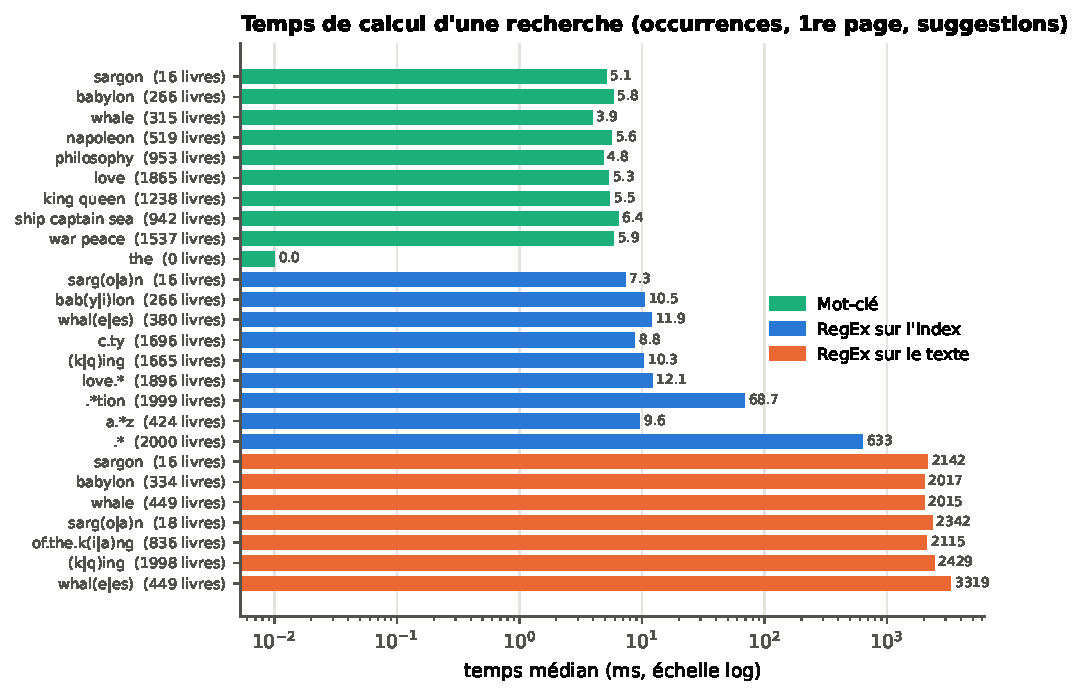
\includegraphics[width=0.78\textwidth]{requetes}
\caption{Temps de calcul d'une requête complète (occurrences, première page
  classée, suggestions) sur les 2000 livres, médiane de 5 mesures, échelle
  logarithmique.}
\label{fig:requetes}
\end{figure}

\paragraph{Les trois recherches.} La figure~\ref{fig:requetes} confirme
l'écart attendu entre le précalcul et le parcours des textes. Une recherche par
mot-clé prend 4 à 6~ms, classement et suggestions compris, qu'elle trouve 16
livres (\motif{sargon}) ou 1865 (\motif{love}) : le coût est dominé par les
allers-retours avec PostgreSQL et le tri des résultats en base. Une requête
faite de mots vides (\motif{the}) ne descend même pas en base. La RegEx sur
l'index coûte 7 à 12~ms tant qu'elle reconnaît peu de termes ; \motif{.*tion}
(69~ms) et \motif{.*} (633~ms, tronquée à 2000 termes) sont bien plus chères à
cause de la requête SQL, qui additionne alors des millions de lignes de
\texttt{occurrence}. La compilation de la RegEx est négligeable : moins de
0,25~ms, pour des DFA minimaux de 1 à 8 états. La RegEx sur le texte coûte 2 à
3,3~s, plusieurs centaines de fois plus que l'index.

\begin{figure}[t]
\centering
\begin{minipage}[t]{0.49\textwidth}
  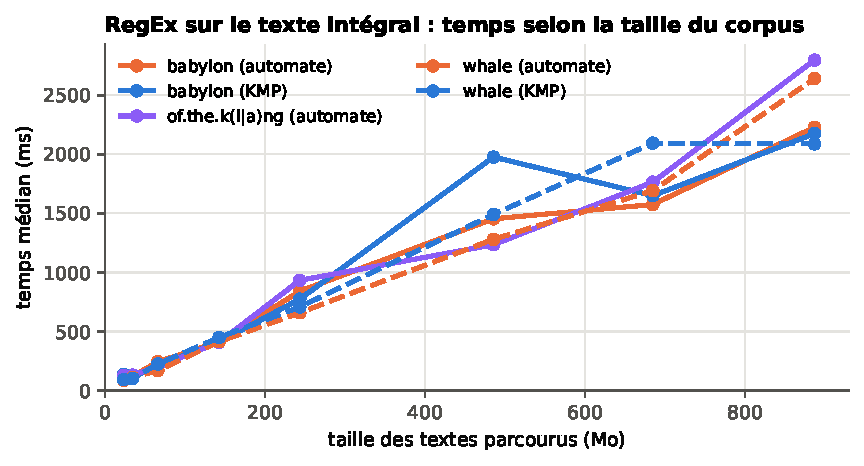
\includegraphics[width=\linewidth]{texte}
  \caption{RegEx sur le texte intégral, en parallèle sur 16 fils : temps
    selon la taille des textes parcourus.}
  \label{fig:texte}
\end{minipage}\hfill
\begin{minipage}[t]{0.49\textwidth}
  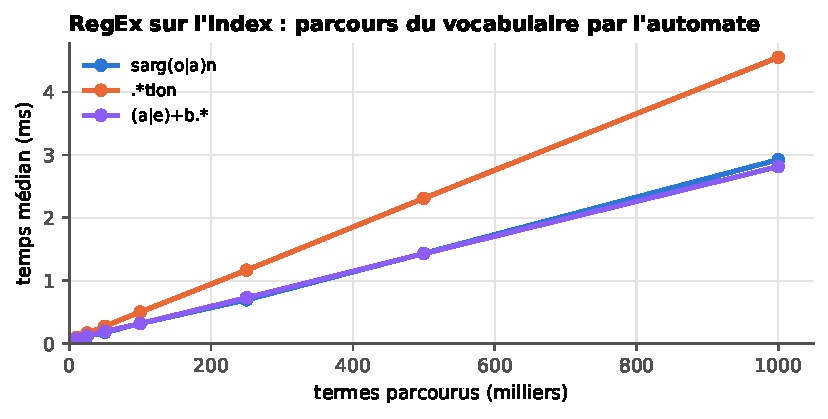
\includegraphics[width=\linewidth]{vocabulaire}
  \caption{RegEx sur l'index : parcours du vocabulaire par le DFA minimal.
    Au-delà des 517\,845 termes du corpus, le vocabulaire est repris en boucle.}
  \label{fig:vocabulaire}
\end{minipage}
\end{figure}

\paragraph{Passage à l'échelle de la RegEx sur le texte.} Le temps croît
linéairement avec la taille des textes lus (figure~\ref{fig:texte}), d'environ
2,5 à 3~ms par Mo : 2,1 à 2,8~s pour les 2000 livres. C'est acceptable pour une
recherche signalée comme lente, mais une seule de ces requêtes occupe tous les
cœurs, d'où le sémaphore. Dans l'API, ni KMP ni l'automate ne l'emporte
nettement : les écarts, jusqu'à 25~\% dans un sens ou dans l'autre selon la
taille, viennent de ce qui est commun aux deux (lecture du disque, décodage
UTF-8, découpage en lignes, mise en minuscules), et la RegEx
\motif{of.the.k(i|a)ng}, qui couvre plusieurs mots, coûte autant qu'un mot
simple. Sur des lignes déjà en mémoire et un seul cœur, l'algorithme
réapparaît : KMP traite 260 à 300 millions de caractères par seconde,
l'automate 175 à 245, car une transition du DFA demande deux accès mémoire (la
colonne de la lettre, puis la case de la table) quand KMP compare le plus
souvent un seul caractère. Le choix du projet~1, KMP dès que la RegEx est un
mot, gagne donc 20 à 70~\%. Avec \motif{the} (745\,391 occurrences), les deux
débits chutent (182 et 144) : le coût vient alors du repérage des occurrences.

\paragraph{Parcours du vocabulaire.} Le test de chaque terme par le DFA est
linéaire en la taille du vocabulaire (figure~\ref{fig:vocabulaire}) : 6 à 11~ms
pour les 517\,845 termes du corpus, 11 à 19~ms pour un million. Pour les RegEx
larges, c'est la requête SQL qui domine, ce qui justifie de ne pas avoir
construit de structure plus élaborée (arbre radix, FST).

\begin{figure}[t]
\centering
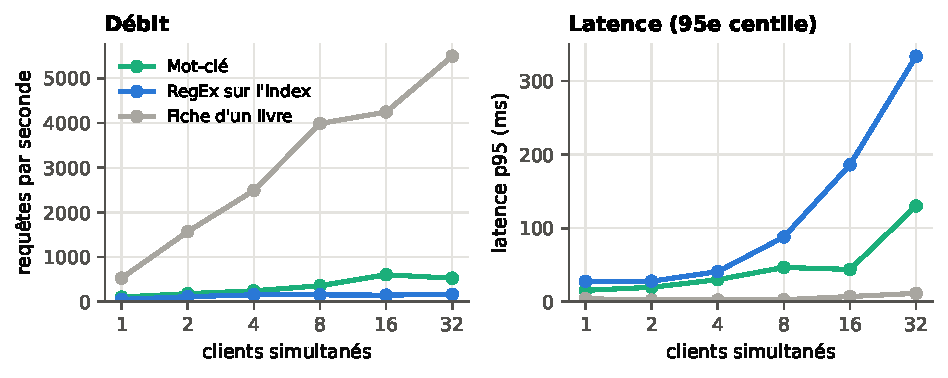
\includegraphics[width=0.8\textwidth]{charge}
\caption{Test de charge de l'API : débit et latence au 95\textsuperscript{e}
  centile selon le nombre de clients simultanés, 10~s par point, aucune erreur.}
\label{fig:charge}
\end{figure}

\paragraph{Test de charge.} Sans erreur sur plus de 210\,000 requêtes, le
serveur sert jusqu'à 5\,500 fiches de livre, 600 recherches par mot-clé et 170
RegEx sur l'index par seconde (figure~\ref{fig:charge}). Le débit du mot-clé
croît jusqu'à 16 clients puis baisse : le client du test et le serveur se
partagent alors les 16 fils de la machine. La RegEx sur l'index plafonne dès 4
clients, vers 155 requêtes par seconde, et sa latence au 95\textsuperscript{e}
centile passe de 28 à 186~ms à 16 clients : son parcours parallèle du
vocabulaire se dispute le même \emph{pool} de fils entre toutes les requêtes.
Sous forte charge, un parcours séquentiel par requête serait préférable, le
parallélisme étant déjà fourni par les requêtes elles-mêmes. Le même test à
travers nginx, dans l'application lancée par Docker, donne des débits du même
ordre (593 recherches par mot-clé par seconde à 16 clients, contre 606) : le
déploiement ne coûte presque rien.
